%!TEX root = ../Thesis.tex
\chapter{Measure permeation enhancement}


\section{Studies to test peptide absorption}
The goal for an oral formulation is to achieve a high bio-availability with low a dosage variance. That is to maximize the percentage of dose absorbed, and to minimize the day-to-day variance. However in order to learn how a formulation attempt may be failing, it is needed to break down the process into individual steps. The typical three steps to consider are dissolution of the tablet, enzymatic stability and permeation enhancement. The first article, \textit{"The role of citric acid in oral peptide and protein formulations: Relationship between calcium and proteolysis inhibition."} \cite{welling2014citric}, included in this thesis is good example of the \textit{in vitro} methods used to evaluate permeation enhancement and enzymatic stability. First the three steps can be understood as a chain. If one link is failing, the overall result will be poor.

Studies to test permeation enhancement ranging from early proof-of-concept development to clinical trials are listed in Figure \ref{typeOfExperiment}. Beyond this list focusing on peptide permeation studies, also dedicated studies of \textit{in vitro} dissolution, peptide stability and toxicology would e.g. be required.

In preclinical development, studies are formally segregated in two categories the \textit{ex vivo} outside the living and the \textit{in vivo} inside the living organism. Often \textit{in vivo} refer to animal studies, not human. The term \textit{in vitro}, in glass [vial], is used instead of \textit{ex vivo}. Speaking of \textit{in silico}, in silicium, is used for computer models. One may feel the latin buzzword terminology has been overly used to a point no longer being \textit{in}. Further there are clinical trials in human. It is obviously sensible to test many new insulin analogues and formulations in fairly inexpensive and fast studies.

Medical research progress by observing relationships and propose general causal mechanisms, that are later verified and utilized. Where clinical trials can be very representative for the intended population of patients, it is difficult to learn exactly why a therapy elicited no positive result. The multiple potential steps of failure cannot be observed. Moreover, negative confirmation is important to narrow in what part of a therapy is essential for a positive outcome. Ethical considerations limit clinical trials to prescribe therapies to not patients in conflict with their best self interest. With \textit{in vivo} studies it is possible to test treatments as long as the animal suffering is kept minimal. Still the gastro-intestinal tract is a complicated machinery and it is not possible to control or measure every aspect the peptide absorption process. Moreover other sources of variance such as the individual variance in animal physiology may introduce noise into measurements. The animal variance makes a step-wise incremental optimization of formulation challenging, as it becomes hard to evaluate what works, due to no significant change of bioavailability. The lab bench \textit{in vitro} experiments offers close to full control of the experiment conditions. These experiments are often fast and of relatively low cost, while the reproducibility and statistical power are high. From a modeling perspective a larger set observations number is needed, especially for non-linear machine learning, see \ref{some section}. Therefore to model in-vitro \textit{in vitro} data is more feasible. The \textit{in vitro} experiments can often be crude and it is accepted as a necessary evil, that the conditions do not exactly represent completely a clinical situation. Figure \ref{typeOfExperiment} listing the range of permeation experiments, is intended reflect this conflict between representative studies and elucidating studies.

When training machine learning models on data from \textit{in vitro} experiments, we only expect the model to reflect the experiment. With a hopefully sufficient theoretical understanding of the overall peptide absorption and the various biases of the \textit{in vitro} experiments, we can hopefully place the model in a context to obtain useful predictions and identify potential causal relationships between formulation and outcome.

\subsection{consider migrate or cut out}
One example is the very recent proposed causal link, that bacteria species \textit{Prevotella copri} and \textit{Bacteroides vulgatus} present in the gastrointestinal tract promote insulin resistance. A broad screening 300 patients, whereof 70 had type-2 diaetes, screened the bacteriome and for 3000 chemical compounds. As later discussed in Section \ref{unbiased_estimation}, any finding selected for being abnormal is no longer unbiased. Especially in setup testing several hypotheses there will be a so called family wise error, where the findings may be due to a sampling uncertainty. Moreover lab-bnech test is needed to confirm the finding, and to confirm actual causal direction of the relationship link. Maybe the life style caused the bacterioum and the insulin resistance. Maybe be the insulin resistance caused the bactorom, and these bacteria are otherwise harmless. Lastly, maybe the bacteria infact are inducing the insulin resistnce. \cite{pedersen2016human}


\subsection{Caco-2 monolayers}
Caco-2 monolayers have been a standard screening method for intestinal drug permeability. The Caco-2 permeation model, as other permeation models, consist of a donor chamber, an epithelial barrier and a receiver chamber. Caco-2 monolayers are colonic human cancer cells, which a much more prolific and easy to handle, than primary (human non-cancer) epithelial cells. When seeded on micro porous filter (Ø 2cm) on a 12-well plate, the Caco-2 cell line will grow and form a epithelial monolayer in two weeks. A typical test will use 4 mono layers per tested treatment and the study is to be repeated on a different day. A concentration of the permeation drug is applied to the donor side, and the receiver side is sampled at 4 time points to measure the diffusion rate. During the test, the nutrient rich growth media is replaced with a minimal buffer solution. The buffer solution only contain a physiological level of electrolytes such as calcium, potassium, sodium, chloride and phosphate plus an acid/base buffer. These ions maintain isotonicity and a normal electrical membrane potential. Active membrane transporter receptors in the epithelial membrane rely on a given correct membrane potential.

Within standard drug development of small molecules, a low permeability result would likely lead to discarding the given analogue, as it is easier to find a new analogue with a favorable permeability. In insulin therapy, there are few alternatives to insulin-like analogues and therefore the low permeability must be alleviated by e.g. co-formulation of permeation enhancers. To use Caco-2 monolayers to test absorption enhancers likely account are smaller part of the use of Caco-2 monolayers. Here the permeability of insulin is already low, and may be increased by a given absorption enhancer. For surfactant enhancers at high concentration, the monolayer can be completely disrupted, while at low concentration no useful effect is observed.

\subsection{Ussing Chamber}
empty

\subsection{Measuring permeability}
To estimate how potent a permeation enhancer is, permeation markers have been used. An obvious marker is human insulin itself, but insulin is difficult to handle and quantification by immunobinding-assay can be expensive. A number of of alternative permeation markers are typically used to compliment insulin. One of these are $^{14}$C or $^3$H isotope labeled mannitol. Mannitol, is approximately as hydrophilic as glucose, and is thought to only diffuse passively via the paracellular pathway through the tight-junctions \cite{anderberg1992epithelial,artursson1994effect}. Unlike glucose, mannitol is not taken up by active transport, and is therefore suitable passive transport marker. As Mannitol is hydrophillic it cannot permeate the lipophilic plasma membrane and can only diffuse between the cells by the tight junctins. Therefore mannitol, is a para-celullular passive permeation marker. Besides permeation of mannitol through the tight junctions, also permeation of electrolytes can be used as a marker of how open the junctions currently are.

Trans epithelial electrical resistance (TEER) can measure how open the para-cellular tight junctions are, as the junction cross sectional area is proportional to the conductivity, and conductivity is inverse resistance. TEER is an non-invasive measurement easy to apply. A certain TEER response can be translated to change of insulin permeability. E.g. lowering the epithelial resistance 50\% by the lauroyl carnitine chloride surfactant enhancer translated to a (40-fold increase) of permeability of insulin in Caco-2 model \cite{welling2014citric}.

FITC-dextran 4000 dalton (FD4) is a florescent labeled sugar polymer of similar hydrophilicity and size as insulin. FD4 can mimic insulin as transport marker as it has the molecular weight and hydropphlicity \cite{vernon1999insulin}. FD4 on the other hand has no enzymatic instability and can be used to estimate what would have been the permeation of unchanged insulin, if the has been no enzymatic cleavage in the luminal space. FD4 can be specifically and accurately quantified, as it is a strong fluorophore.

\begin{figure}[!htpb]
\label{devel_typeOf}
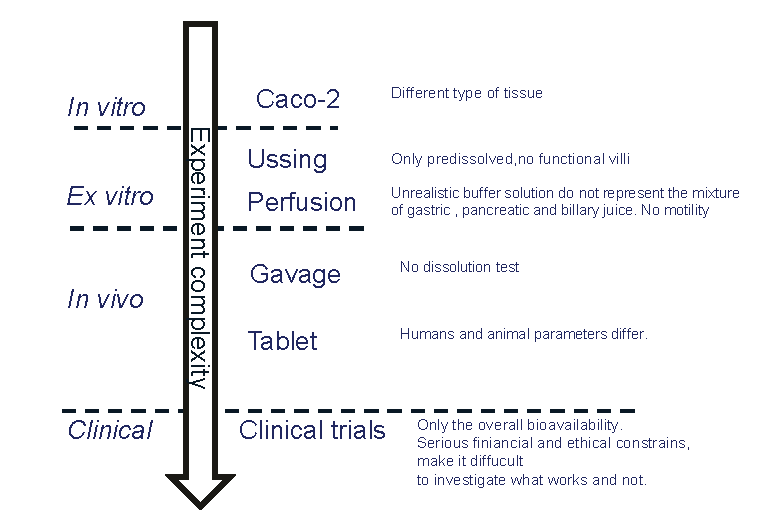
\includegraphics{graphics/typeOfExperiments.pdf}
\caption{Schematic overview of types of experiments ranging from Caco-2 to clinical. Simple experiments to not accurately simulate the actual process, and there will be a number of biases which must not be over interpreted.}
\end{figure}

\subsection{Calculating permeability}
Gradient driven diffusion of mannitol, FD-4 and insulin across the epithelial barrier is a first order process, where the transport per time (aka. flux) is proportional to the concentration gradient $C_i$ ($mol/L$). Only a few percent of the total amount of transport marker will permeate the barrier and therefore will $C_i$ be approximately unchanged throughout the experiment. Hereby becomes the apparent permeability $\bm{P}_{app}$ proportional to the transport rate or flux $\bm{J}$ ($mol/s$) which is usually estimated by sampling the reciever basolateral side 4 to 6 times. When plotting receiver concentration versus time, a fitted ordinary least squares slope is used as the overall transport rate through out the experiment. Permeability is the flux, per concentration gradient and cross sectional area of the chamber, $\bm{A}$ ($cm^2$). Therefore the apparent permeability is calculated as

$\bm{P}_{app} = \bm{J} / \bm{A} / \bm{C}_i = \frac{d\bm{C}_r}{dt} / \bm{A} / \bm{C}_i \quad ,$

where $\frac{d\bm{C}_r}{dt}$ is the slope of ordinary least squares regression of receiver chamber concentration versus time. The intercept with x-axis (time) is interpreted as the lag time, which is the time it takes to saturate the mucus layer, the thin unstirred water layer and the epithelial junctions. The lag time is typically a couple of minutes depending weather using Caco-2 or Ussing chamber. To observe an apparent constant flux e.g. throughout a one hour experiment is normal. The small decrease in concentration gradient of some few percent throughout the study may theoretically have caused deceleration of the flux. However, it is possible that the actual permeability of the epithelial barrier is increasing through the one hour flux study due to slow deterioration by the absorption enhancer, and therefore a constant flux is observed. In control epithelial barriers without absorption enhancer treatment, the barrier integrity is not expected to decline, but at the same time the flux is very low, so the concentration gradient do not change.

\begin{figure}[!htpb]
\label{meassure_TEERPapp}
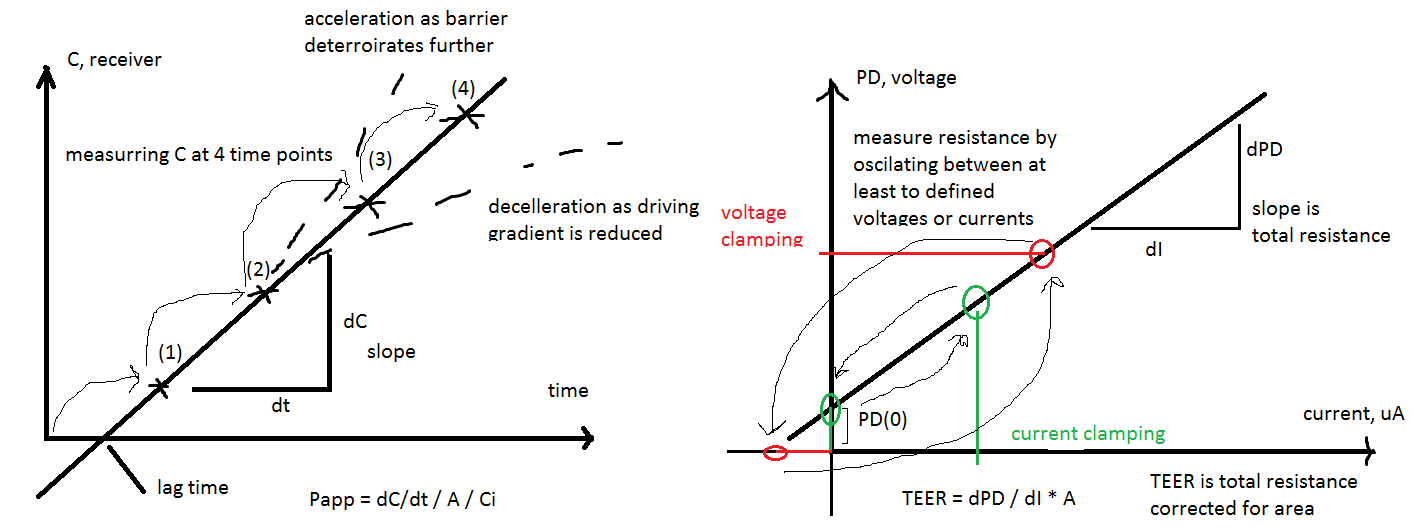
\includegraphics[width=\textwidth,height=\textheight,keepaspectratio]{graphics/sketch_measuring_permeability.png}
\caption{Illustration of how \textit{(a)} $\bm{P}_{app}$ and \textit{(a)}  TEER is calculated.}
\end{figure}

The tight junctions in ideally water filled channels between the cells of the barrier. The water in the channels can be thought to have specific conductance depending on the concentration and diffusability of ions. When tight junction are widened, the cross-sectional area of tight-junction is changed. Similarly as marker transport is driven by a concentration difference, the electrical current $\bm{I}$ (Ampere $\mu A$) is driven by an electrical potential difference $\bm{U}$ (Voltage $V$). The electrical current $\bm{I}$ is analogue to $\bm{J}$ and potential difference $\bm{U}$ to $\bm{C_i}$. Therefore the membrane conductivity corrected for membrane area $\bm{G_A}$ area can be expressed in parallel to $\bm{P_{app}}$, such that

$\bm{G_A} = \bm{I} / \bm{A} / \bm{U} \quad .$

The inverse of $\bm{G_A}$ is named TEER (trans epithelial electrical resistance)(Ohm cm$^2$) in drug transport studies. To summarize both $\bm{P_{app}}$ and inverse TEER both describe how readily a flux of either molecules or ions are driven through the epithelial barrier by respectively a concentration gradient or a electrical potential gradient.

Figure \ref{meassure_TEERPapp} describes how to calculate the slopes for $P_{app}$ and TEER. For $P_{app}$  the receiver concentration $\bm{C}_r$ is plotted as a function of time, the slope represents flux $\bm{J}$. TEER is either measured with voltage or current clamping. To measure TEER with voltage clamping is to control the electrical gradient (potential difference) with electrodes and measure the actual current. Whereas, current clamping is to drive a specified flux of ions (current) through the epithelial barrier and record the electrical gradient. In either case is the membrane potential difference $U$ plotted as a function of current. The slope represents TEER not corrected for area. At zero applied current, the potential difference is not neccesarily zero, as the epithelia has an active energy dependent ion transport.

For direct measurement of the intrinsic permeability of a given drug molecule without permeation enhancers, TEER is mainly used to check barrier integrity. For measuring the potency of permeation enhancers to increase permeability, TEER can be used as indicator hereof. To directly measure the permeation of insulin would be preferable, but this is more slow, expensive and unlikely to in already published results. As the current and potential difference can be manipulated with electrodes, the time resolution for TEER measurements are ideally in seconds. The time resolution for permeation markers is limited by the sampling rate and accuracy of the concentration determination. However, in Caco-2 studies the sampling rate for both TEER and $\bm{P}_{app}$, the sampling rate of Caco-2 studies are typically once per 15 minutes.

\section{Mechanisms of absorption enhancement in oral formulations}
The formulation part of oral peptide therapy is mainly to ferry the highest possible total and relatively amounts of insulin unchanged through the upper gastro-intestinal tract. The two major barriers are enzymatic degradation and poor epithelial permeability. Other barriers are the mucus and thin unstirred water layer on top of the epithelia. These barriers are not regarded as prominently rate limiting bottle necks and are not given as much attention.(cite)

\subsection{Preventing and measuring enzymatic degradation}
Enzymatic stability of peptides vary greatly in the intestinal tact. From dissolution in the small intestinal lumen the window is concidered to be from a single minutes upto 15 minutes(citation somastatin). Enzymatic degradation rate ($V_i$) is assumed to follow Michalis-Menten kinetics. Describing the degradation rate per enzyme as a function of substrate/peptide concentration $[S]$, enzyme-substrate binding constant ($K_m$), and max enzyme degradation speed $V_max$.

$V_i = \frac{V_{max} [S]}{K_{M}+[S]}$

The Michales-Menten kinetics describe that at very low concentrations of substrate the degradation rate will be proportional to the concentration of insulin in the luminal space, thus a first order decay process. 
The Michaelis-Menten kinetics opens for three ways to limit relative peptide degradation. First the apparent $K_m$ binding constant can be increased by adding a competitive substrate. The enzyme will then bind to another substrate such as soy bean peptides or Bowman-Birk compounds. A very potent non competitive inhibitor would bind strongly to the enzyme, such that only a small amount of inhibitor would be needed. Such non-peptide inhibitors are in practice toxic and not suited for chronic treatment \cite{bernkop1998use} \cite{murthy1980effect}. 

The second option which is used in the first article \cite{welling2014citric} of this thesis is to lower the apparent $V_max$ the intrinsic fastest rate of enzyme conversion. Citric acid itself is not a substrate of the trypsin and chymotrypsin. As citric acid is dissolved, it will partly release protons into the luminal space and thereby lower pH. The enzymes trypsin and chymotrypsin has an 10-fold lower $V_max$ at pH=4.
The last way to inhibit the relative degradation is to release as much substrate as fast as possible into the luminal space. As the substrate concentration increase $[S] >> K_m$ and $V_i \approx V_{max}$ there will be a theoretical upper limit for how much insulin can be degraded per time. Driving up the concentration of insulin, will surpass the linear range of degradation and approach the $V_max$. This approach could fairly be called hit and run, as when to release enough insulin in such a short time and location, that the enzyme cannot degrade all at once. The latter approach is highly connected to the dissolution of the tablet. If the tablet disolves over an hour. The insulin would be released very slowly in small concentrations, and the enzymes will have plenty of opportunity to degrade all insulin. To simply only drive up the amount of insulin included in a tablet is not likely to be the solution alone, as the insulin is very costly to produce. Also, due to drug safety, there can be a upper boundary of how much insulin, that can be included in one tablet, as it may lead to an overdose and acute hypoglychemia, if suddenly a large fraction insulin was absorbed in patient.


\subsection{Citric acid, a calcium chelator}
maybe include


\newpage

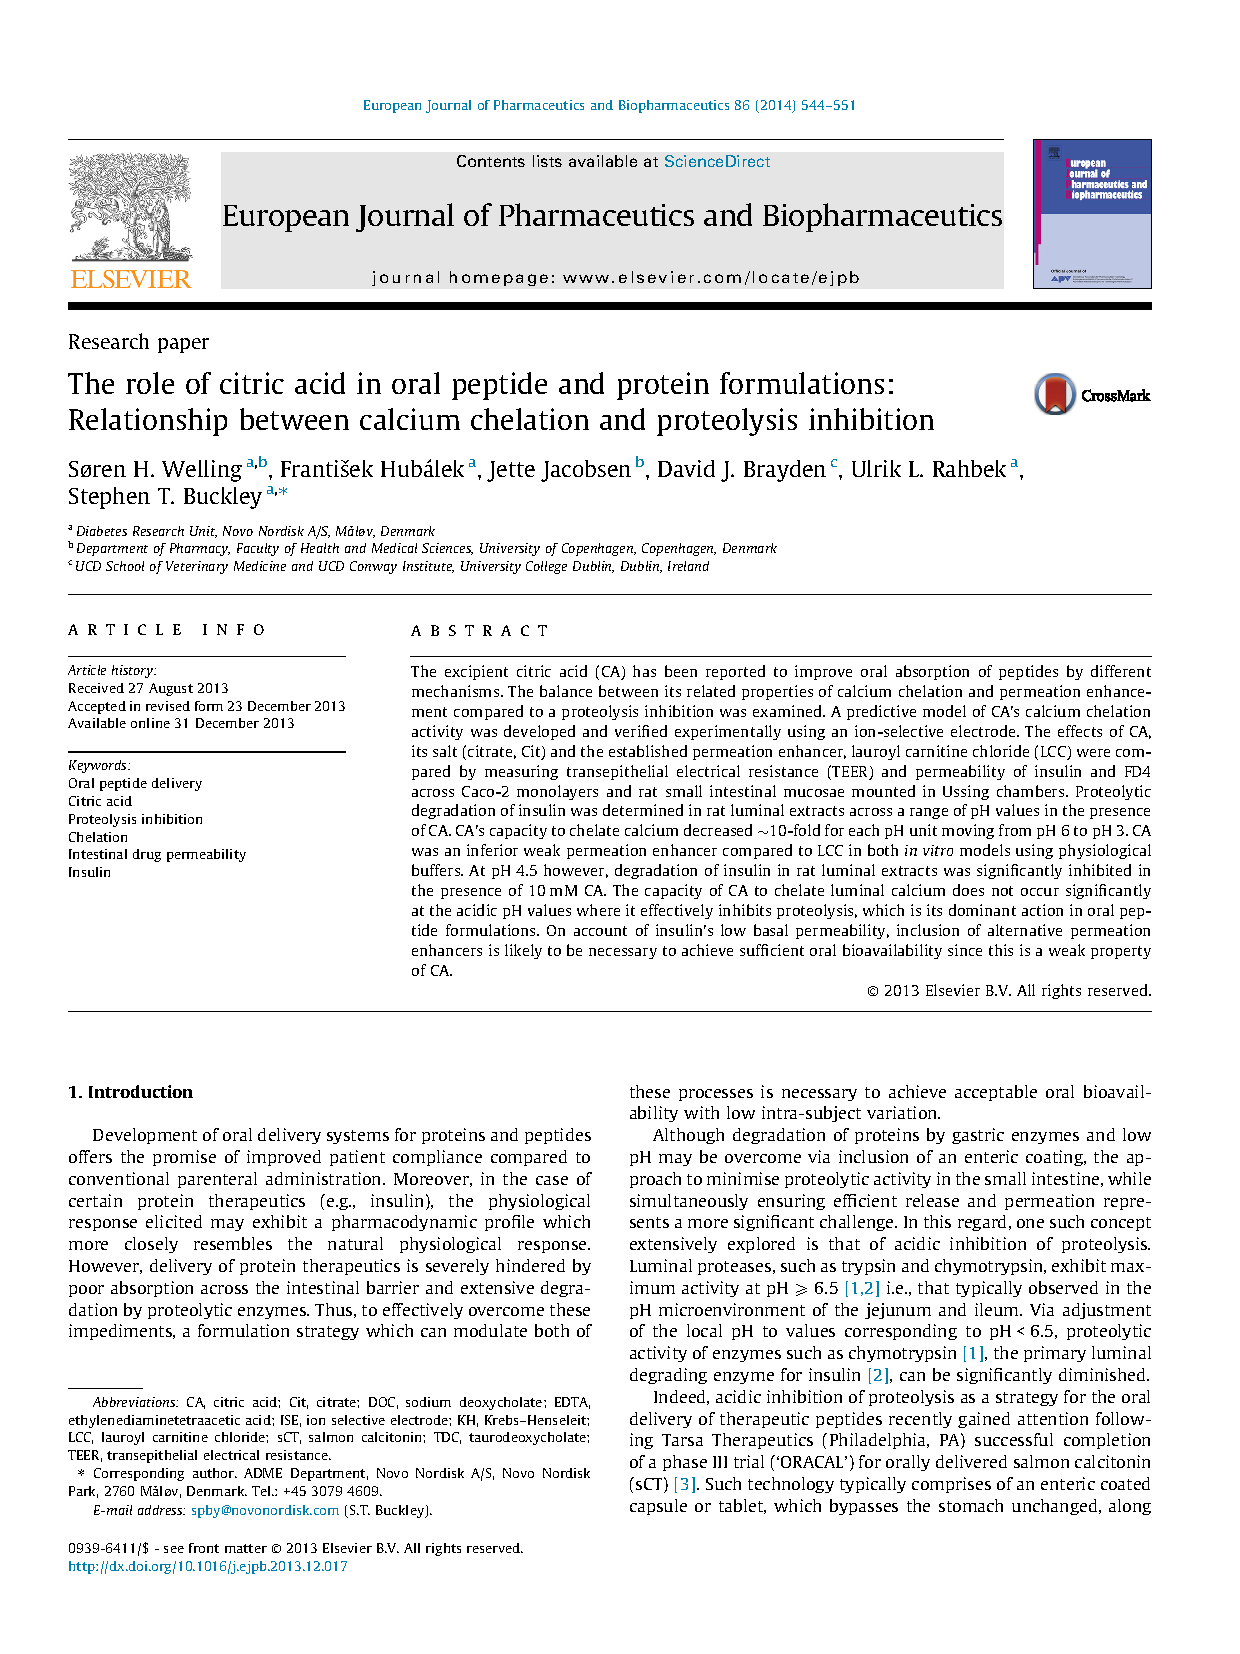
\includepdf[pages={1-},scale=0.90,pagecommand={\pagestyle{myruled}}]{chapters/citricAcid.pdf}